\documentclass[a4paper]{article}
\usepackage[spanish]{babel}
\title{Trabajo Práctico 1}

\usepackage[utf8]{inputenc}
\usepackage{caratula}
\usepackage{graphicx}
\usepackage{color}
\usepackage{listings}
\usepackage{float}

\setlength{\leftmargin}{2cm}
\setlength{\rightmargin}{2cm}
\setlength{\oddsidemargin}{-1cm}
\setlength{\evensidemargin}{-1cm}
\setlength{\topmargin}{-1cm}
\setlength{\textwidth}{18cm}
\setlength{\textheight}{25cm}

\usepackage{fancyhdr}
\pagestyle{fancy}
\fancyhf{}
\fancyhead [LO,LE]{\scriptsize Trabajo Práctico N$^{\circ}$1}
\fancyhead [RO,RE]{\scriptsize Mancuso, Mataloni, Tolchinsky}
\fancyfoot[CE,CO]{\thepage}
\renewcommand{\footrulewidth}{0.4pt}

\usepackage[pdftex, bookmarks=true, colorlinks, citecolor=black, linkcolor=black]{hyperref}
\usepackage{multirow}

\begin{document}

\materia{Métodos Numéricos}
\submateria{Primer Cuatrimestre de 2012}
\titulo{Aproximación de Ceros o Raíces de una función. }
\subtitulo{ Aproximación Numérica,  Bisección, Newton-Raphson }
\grupo{Trabajo Práctico N$^{\circ}$1}

\integrante{Mancuso, Emiliano}{597/07}{emiliano.mancuso@gmail.com}
\integrante{Mataloni, Alejandro}{706/07}{amataloni@gmail.com}
\integrante{Tolchinsky, Lucas}{591/07}{lucas.tolchinsky@gmail.com}

\maketitle

\begin{verse}
\abstract{
%El resumen, de no más de 200 palabras, debería explicar brevemente el trabajo realizado y las conclusiones de los autores de manera que pueda ser u ́til por s ́ı solo para dar una idea del contenido del trabajo. Las palabras clave, no m ́as de cuatro, deben ser t ́erminos t ́ecnicos que den una idea del contenido del trabajo para facilitar su bu ́squeda en una base de datos tem ́atica.

El trabajo implementa un programa que permite aproximar la raíz de una función por los métodos de \textbf{Bisección} y \textbf{Newton-Raphson}, utilizando para esto aritmética de punto flotante variando la precisión de la mantisa, hasta un máximo de 52 bits. En cuanto a la calidad de resultados ambos algoritmos nos proporcionan la misma precisión, sólo que \textbf{Newton} lo hace con un orden de convergencia cuadrático (contra el lineal de \textbf{Bisección}). Sin embargo, éste necesita una \textit{semilla} inicial cercana a la raíz buscada para asegurar la convergencia, por lo que decidimos implementar una combinación de ambos, aplicando primero \textbf{Bisección} para encontrar un punto inicial cercano, y luego aplicar \textbf{Newton} desde la semilla encontrada.  
}
\end{verse}


\newpage

\addcontentsline{toc}{section}{Índice}
\tableofcontents

% Main project

\newpage

\section{Introducción Teórica}
%Contendr ́a una breve explicaci ́on de la base te ́orica que fundamenta los m ́etodos involu- crados en el trabajo, junto con los m ́etodos mismos. No deben incluirse demostraciones de propiedades ni teoremas, ejemplos innecesarios, ni definiciones elementales (como por ejemplo la de matriz sim ́etrica). En vez de definiciones b ́asicas es conveniente citar ejemplos de bibliograf ́ıa adecuada. Una cita vale m ́as que mil palabras.
Sea $f(x)$ una función, un problema interesante a resolver es el de encontrar todos los $x$ pertenecientes al dominio de $f$ tal que $\mathbf{f(x) = 0}$. Para resolver este problema se conocen varias técnicas que utilizaremos en este trabajo. \\
Supongamos que el dominio de $f$ son los números reales. Dado que vamos a resolver el problema con una computadora nos encontramos frente al primer inconveniente. Las máquinas tienen una cantidad acotada de bits para representar los números. Es por esto que no todos los números pueden ser representados, por ejemplo $\sqrt(3)$ no puede ser representado ya que es irracional y tiene infinitas cifras decimales. Es por esta razón que los algoritmos no pueden dar una solución exacta a este problema, aunque si lo bastante cercana a la misma para que sea aceptable en la mayor parte de las situaciones. 
  
\subsection{Bisección}
También conocido como método de \textbf{Búsqueda binaria}, se basa en el teorema del valor intermedio \footnote{  p10 \textbf{Análisis Numérico} - Burden, Faires. 7ma edición. }. 
Requiere dividir varias veces a la mitad los subintervalos de [a,b] y, en cada paso, localizar la mitad que 
contenga a \textbf{p}, tal que $\mathbf{f(p) = 0}$.
Si bien tiene una importante propiedad, que asegura la convergencia en una solución, 
esta convergencia puede ser muy lenta. 
Por eso, a menudo se utiliza para iniciar otros métodos mas eficientes, como por ejemplo \textbf{Newton-Raphson}.

\subsection{Newton-Raphson}
El \textbf{método de Newton-Raphson} es una de las técnicas más eficientes para calcular ceros de función,
dado que nos provee convergencia cuadrática. El método precisa de un $\mathbf{x_0}$ cercano 
al \textbf{p} tal que $\mathbf{f(p) = 0}$ y la ecuación del mismo se inspira en el desarrollo de
Taylor de grado dos alrededor de $\mathbf{x_0}$:

$$f(x) = f(x_0) + (x - x_0)f'(x_0) + \frac{(x - x_0)^2}{2}f''(x_0)$$
Evaluando en \textbf{p}:
$$0 = f(x_0) + (p - x_0)f'(x_0) + \frac{(p - x_0)^2}{2}f''(x_0)$$
Como  $|p - x_0|$ es muy chico $(p - x_0)^2 \approx 0$, luego:  
$$0 \approx f(x_0) + (p - x_0)f'(x_0)$$
$$p \approx x_0 - \frac{f(x_0)}{f'(x_0)}$$

De esta manera, podemos generar la serie $x_{n + 1} = x_n - \frac{f(x_n)}{f'(x_n)}$ que, arrancando de un $x_0$ adecuado, converge a \textbf{p}.

\newpage

\section{Desarrollo}
%Deben explicarse los m ́etodos num ́ericos que utilizaron y su aplicaci ́on al problema concreto involucrado en el trabajo pr ́actico. Se deben mencionar los pasos que si- guieron para implementar los algoritmos, las dificultades que fueron encontrando y la descripci ́on de c ́omo las fueron resolviendo. Explicar tambi ́en c ́omo fueron planteadas y realizadas las mediciones experimentales. Los ensayos fallidos, hip ́otesis y conjeturas equivocadas, experimentos y m ́etodos malogrados deben figurar en esta secci ́on, con una breve explicaci ́on de los motivos de estas fallas (en caso de ser conocidas).

Nuestro objetivo consistía en calcular el momento de impacto de un cuerpo, lanzado desde una altura \textbf{h} y a una velocidad inicial \textbf{$v_0$}. Dada la ecuación de la posición de un cuerpo en un instante \textbf{t}

\begin{equation}
 y(t) = h + v_0 t - \frac{g}{2} t^2,
\end{equation}

nuestro trabajo se reducía a encontrar los instantes en que esta función vale cero, y esto se transforma en calcular las raíces o ceros de la función. Para esto utilizamos los métodos numéricos de \textbf{Bisección} y \textbf{Newton}.

Como las condiciones de convergencia de \textbf{Newton} exigen que la semilla este \textit{cerca} de la raíz, decidimos implementar la combinación de los mismos, es decir conseguir una \textit{semilla} con el método de \textbf{bisección} y luego utilizar la misma para aplicar \textbf{Newton}. \\ \hspace{1em}

En el punto dos, para calcular la altura máxima luego del primer rebote podemos aplicar el mismo razonamiento y calcular la raíz de la función velocidad

\begin{equation}
 \dot{y}(t) = v_0 - g t
\end{equation}

con los parámetros iniciales correspondientes. Con esta raíz, que es el instante \textbf{t}, la utilizamos para calcular la posición del cuerpo y así obtener la altura máxima luego del primer impacto ya que ésta se corresponde con el momento en que el cuerpo tiene velocidad nula.\\ \hspace{1em}

Para calcular el segundo impacto, volvemos a calcular el cero a la función posición,  actualizando los parámetros iniciales. Que son 

\begin{itemize}
 	\item $V_0 = -f_r *V_{impacto} $
	\item $h = 0$ 
\end{itemize}

O sea, lo que hacemos es tirar el cuerpo desde una altura $V_0$ con una velocidad igual a la contraria con la que llego al piso multiplicada por el correspondiente factor de rozamiento. La raiz de la función posición con estos parámetros iniciales se corresponde con el instante en el que el cuerpo impacta con el piso por segunda vez.

\hspace{1em}

Básicamente, el trabajo consiste en calcular o aproximar ceros de distintas funciones y por eso decidimos implementar una función genérica para cada algoritmo, que recibe como parámetro la función a la cual se le quiere aproximar las raíces. 

En un principio utilizamos el tipo \textit{double} para asegurarnos de que todo funcionaba según lo esperado. Luego fue reemplazado por la clase \textit{TFLoat} proporcionada por la cátedra, con la cual íbamos a poder manejar la cantidad de bits de la mantisa.   
Un error que se nos presentó fue justamente el de la presentación de la información. Al imprimir los valores de las variables, imprimimos pocos decimales, estos eran redondeados dandonos valores alejados de lo esperado. Para saber la cantidad máxima de dígitos consultamos la clase $float.h$\footnote{http://www.cplusplus.com/reference/clibrary/cfloat/} la cual contiene una constante que indica el número de decimales significativos. \\[1em]

Dado que ambos métodos son iterativos, y bajo ciertas circunstancias nos aseguran una convergencia a la solución, debíamos proveer de un criterio para saber cuando nos encontramos con una 'buena' aproximación a la solución. Como no podemos preguntarle a una computadora si un valor es exactamente igual a 0, nos conformarnos con una aproximación al mismo.

Siendo $\epsilon$ una tolerancia previamente establecida (por ejemplo $\epsilon = 10^{-3}$), uno de los criterios de parada consiste en parar cuando 
\begin{equation}|f(c_n)| < \epsilon \end{equation}
También se puede usar como criterio de parada el error relativo entre dos aproximaciones del cero de f, 
\begin{equation}\frac{c_n - c_{n-1}}{c_n} < \epsilon \end{equation}
Otro criterio que puede utilizarse, y de hecho es el que utilizamos, es examinar sí \begin{equation}\vert{b_n - a_n}\vert < \epsilon\end{equation} siendo $b_n$ y $a_n$ los bordes del intervalo.

En el caso de \textit{Newton} utilizamos el mismo criterio, aplicado a dos iteraciones consecutivas del método. \begin{equation}\vert{p_n - p_{n-1}}\vert < \epsilon\end{equation}





Este criterio de parada lo elegimos por ser el más simple, más adelante evaluamos la importancia del $\epsilon$. Ver \texttt{Tabla 1}.

\newpage

\section{Discusión y Resultados}
\begin{quote}
Salvo para las pruebas de precision, \texttt{Figura 6}, utilizamos la mayor precision que podíamos dada por \textbf{TFloat}, que es 52bits.
\end{quote}
\vspace{1em}

Sabiendo que el método de \textbf{Newton-Raphson} converge de forma cuadrática, decidímos comparar la cantidad de iteraciones que requiere cada algoritmo para mostrar de forma gráfica la eficiencia de los mismos. \\

Para esto, nos centramos en resolver el problema con parámetros fijos de solución exacta.

\subsection{Casos de prueba}
 Creamos dos configuraciones distintas para utilizar en los resultados que describimos a continuación.
Elegimos estas configuraciones porque podemos obtener resultados exactos analíticamente y nos facilita comparar los resultados de nuestro algoritmo con los reales.

\subsubsection{Configuración A} 
\begin{itemize}
  \item{G = 9.81}
  \item{Velocidad Inicial = 29.43 (3G)} 
  \item{Altura Inicial = 78.48 (8G)} 
  \item{Tolerancia = $10^{-14}$} 
  \item{Máx. Iteraciones = $10^5$}
\end{itemize}

\subsubsection{Configuración B}
\begin{itemize}
  \item{G = 9.81}
  \item{Velocidad Inicial = 0.0} 
  \item{Altura Inicial = 19.62 (2G)} 
  \item{Tolerancia = $10^{-14}$} 
  \item{Máx. Iteraciones = $10^5$}
\end{itemize}

\newpage

\subsection{Experimentación}
Las \texttt{Figuras 1, 2 y 3} representaran los resultados con la \texttt{configuración A}.
Bajo estas condiciones, es fácil probar que la solución es exactamente 8, basta con resolver la siguiente ecuación cuadrática:

\begin{displaymath}
  \frac{-3G \pm \sqrt{9G^2 + 4*\frac{G}{2}*8G}}{-2\frac{G}{2}}
\end{displaymath}

Ahora, con este problema bien definido, variamos la longitud del intervalo donde comienza \textbf{bisección} y graficamos la cantidad de iteraciones que necesita cada algoritmo (\texttt{Figura 1}).

\begin{figure}[H]
  \centering
  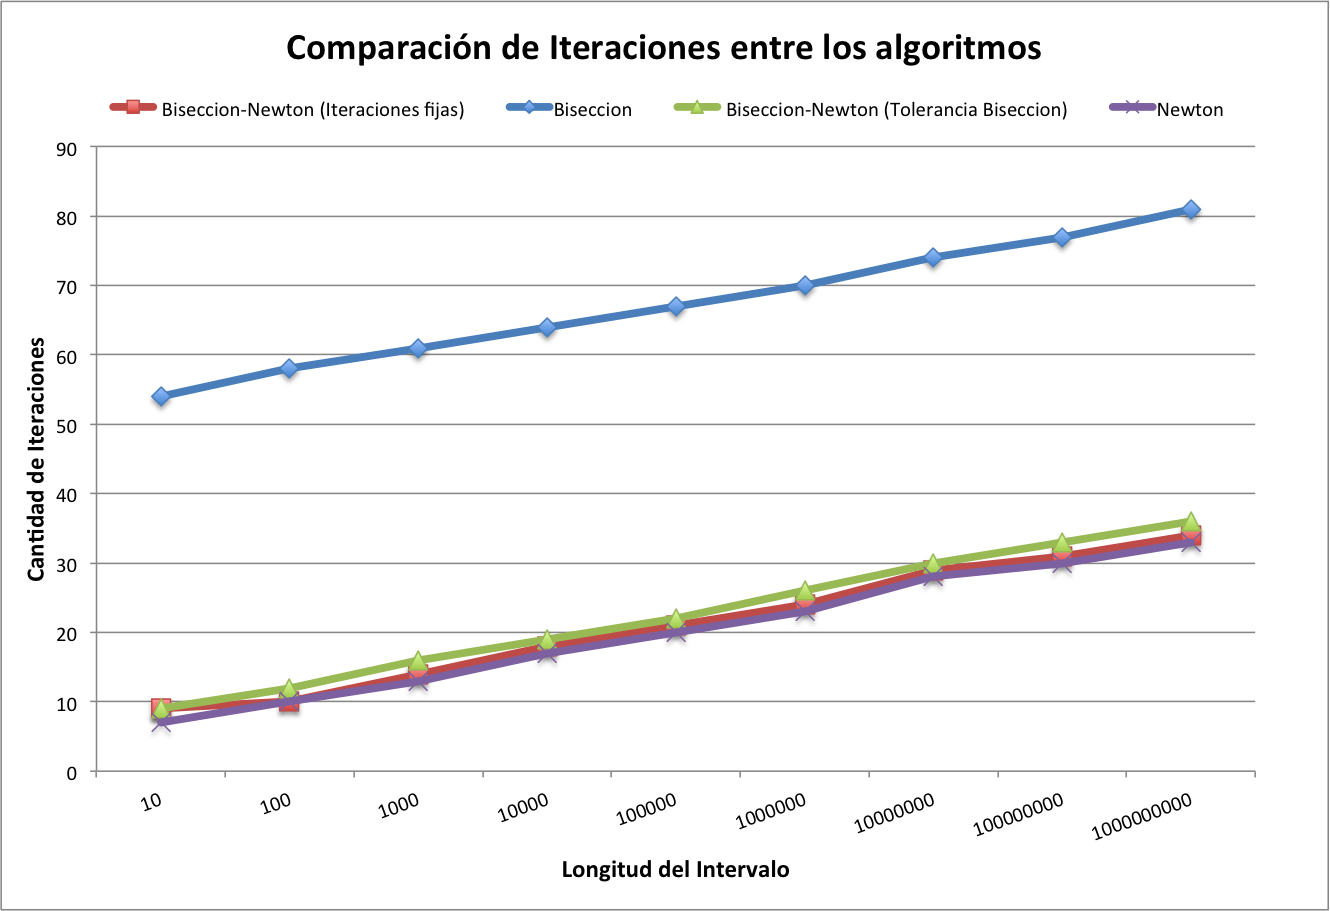
\includegraphics[scale=0.80]{graficos/1-Biseccion_vs_BiseccionNewton.png}
  \caption{Cantidad de Iteraciones. Bisección vs Newton (con aproximación de Bisección) }
\end{figure}

En primer lugar, encontramos una gran diferencia entre la cantidad de iteraciones necesarias por parte de \textbf{Bisección puro} y \textbf{Bisección + Newton}. Este resultado ya lo sabíamos teóricamente con el orden de convergencia de ambos métodos y quedó demostrado. Cabe destacar que no solo probamos este caso en particular sino todas las pruebas que fuimos haciendo verificábamos esto.\\[1em]
 

Por otro lado , necesitábamos un criterio de aproximación por \textbf{Bisección} para la semilla de \textbf{Newton}, y decidímos probar las 2 alternativas:
\begin{itemize}
  \item Iterar una cantidad fija de veces
  \item Acercarnos al valor a una distancia \textbf{d} de la raíz
\end{itemize}

\begin{figure}[H]
  \centering
  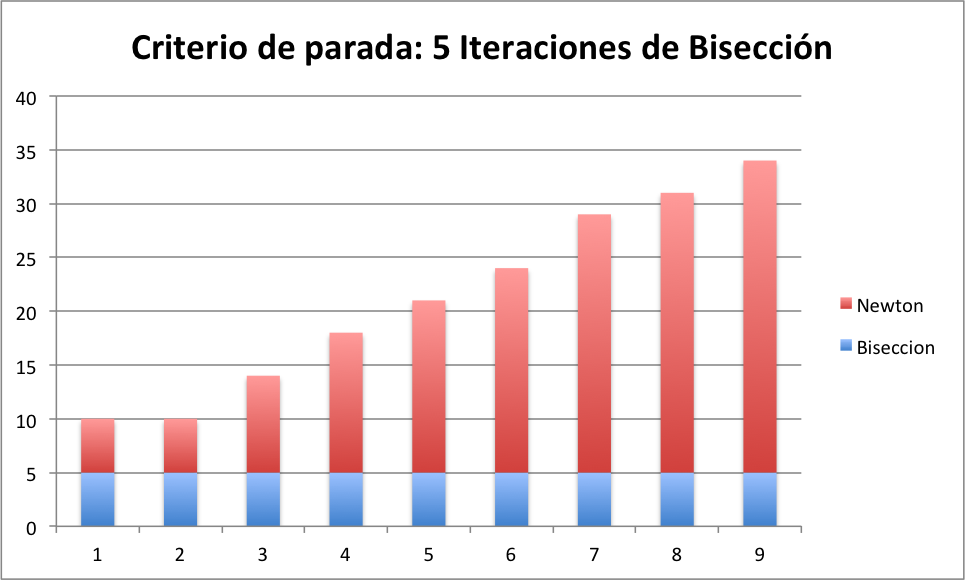
\includegraphics[scale=0.80]{graficos/2-BiseccionXIteraciones.png}
  \caption{Aproximación con Bisección limitada a 5 iteraciones. }
\end{figure}
 
\begin{figure}[H]
  \centering
  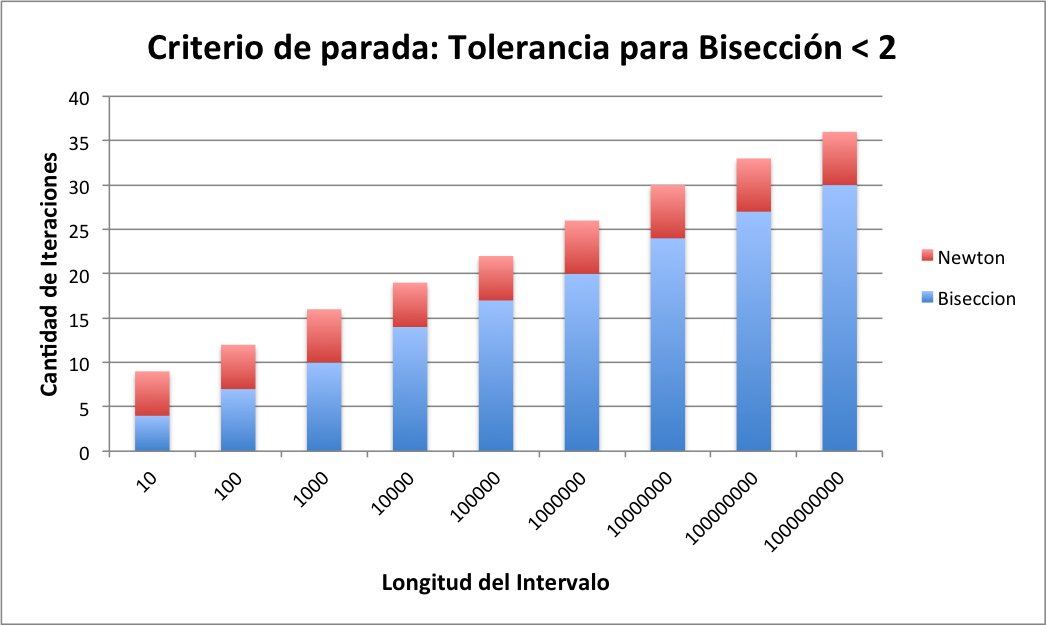
\includegraphics[scale=0.80]{graficos/3-BiseccionXTolerancia.png}
  \caption{Aproximación con Bisección limitada a una tolerancia de 2. }
\end{figure}

En la \texttt{Figura 2 y 3} podemos observar que es ligeramente mejor utilizar iteraciones fijas sobre \textbf{Bisección} pues no varia mucho la cantidad final de iteraciones para encontrar la raíz. En estas figuras, también diferenciamos la cantidad de iteraciones de cada método, y dado que para este problema en particular \textbf{Newton} se comporta \textit{bien} para una semilla aleatoria, decidimos utilizar una cantidad fija de iteraciones.
En el caso de un problema en que sea necesario tener una semilla buena, se optaría por el otro criterio de parada.
Este fue uno de los resultados que nos sorprendió, ya que esperábamos que acercarse a una distancia \textbf{d} de la raíz, nos iba a aportar muchas más iteraciones de las experimentadas.

\newpage

En la siguiente tabla, mostraremos como realmente afecta la elección de la tolerancia al momento de obtener resultados. Esto queda explícito cuando buscamos el instante del primer impacto, ya que sabemos que la posición debería ser cero y analíticamente el instante de impacto ocurre a los 8 segundos. Como se puede observar, los resultados mas cercanos los obtenemos con tolerancias realmente chicas.
Es muy importante la buena elección de la tolerancia, quizás no en aplicaciones como estas que no hay riesgo, pero errores de este tipo en aplicaciones que deben ser precisas (como el disipador de un reactor nuclear) pueden ser muy costosos.

\vspace{2em}
\begin{center}
\begin{tabular}{|l|l|l|}
  \hline
  Tolerancia & Instante (segundos) & Posición \\
  \hline
  2 & 8.875000000000000 & -46.674140624999950 \\
  1 &  8.312500000000000 & -15.807128906250000 \\
  0.5 & 8.031250000000000 & -1.537602539062505 \\
  0.1 & 7.960937500000000 & 1.908531188964787 \\
  0.01 & 8.004882812500000 & -0.239618897438106 \\
  0.001 & 7.999938964843750 & 0.002993756141507 \\
  0.0001 & 8.000007629394531 & -0.000374222087260 \\
  0.00001 & 7.999999046325684 & 0.000046777720740 \\
  0.000001 & 7.999999582767487 & 0.000020465253954 \\
  0.0000001 & 8.000000052154064 & -0.000002558156893 \\
  0.00000001 & 7.999999993480742 & 0.000000319769583 \\
  0.000000001 & 8.000000000291038 & -0.000000014275486 \\
  0.0000000001 & 7.999999999963620 & 0.000000001784485 \\
  0.00000000001 & 8.000000000004547 & -0.000000000223054 \\
\hline
\end{tabular}
\end{center} 
\centerline{Los valores de esta tabla corresponden a la \texttt{Configuración B}. }
\vspace{1em}

%En este caso debíamos analizar cómo variaba la energía mecánica entre el lanzamiento y el segundo rebote.
	
Más adelante, \texttt{Figura 4}, comparamos la energía mecánica a través del tiempo. En este primer experimento dejamos fijo el factor de restitución y variamos la variable $\alpha$  ( $\alpha = 0$ significa sin rozamiento ). Podemos observar que en el caso de no haber rozamiento la energía mecánica se conserva, en cambio a mayor $\alpha$, o sea a mayor rozamiento, la perdida de energía es mayor con el paso del tiempo. \\

\begin{figure}[H]
  \centering
  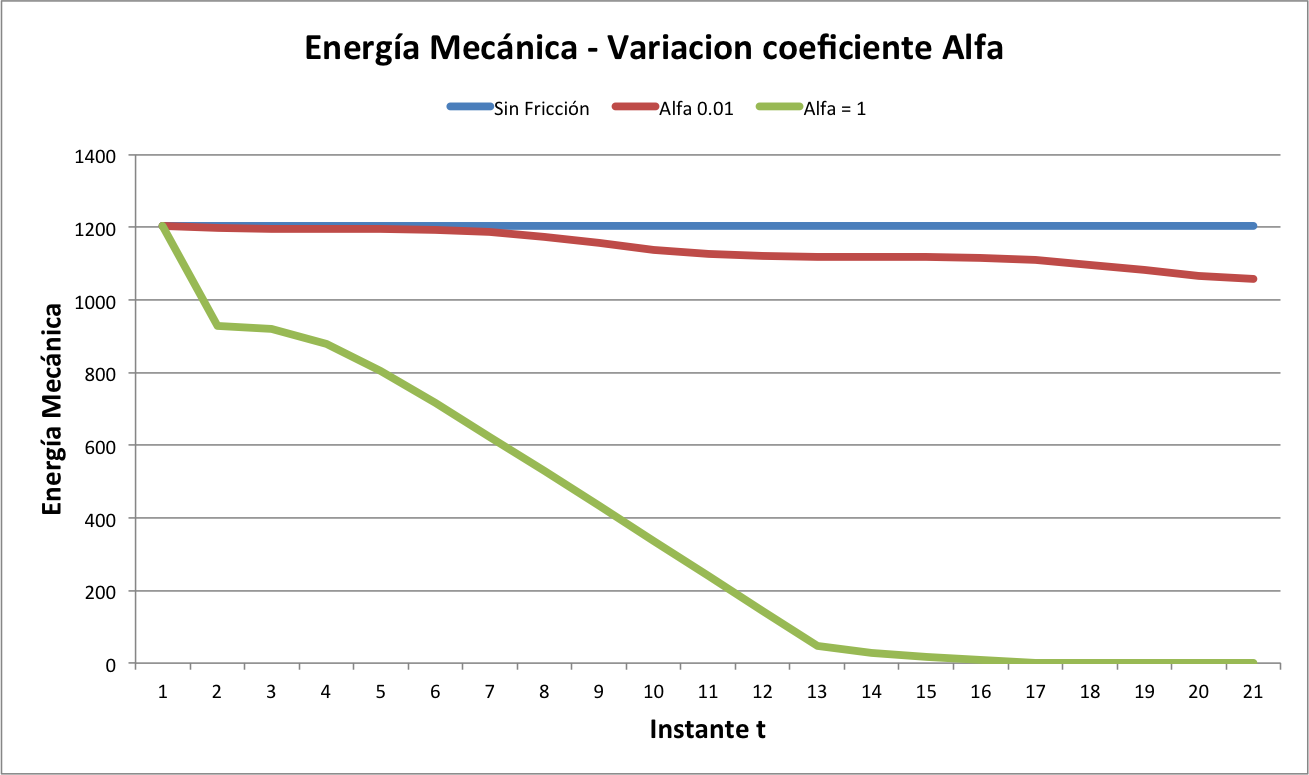
\includegraphics[scale=0.75]{graficos/4-energiaMecanica-alpha.png}
  \caption{Comparación diferencia de energía mecánica. Variando $\alpha$ }
\end{figure}

Los cambios bruscos que podemos ver en los gráficos, se corresponden con los momentos de impacto del cuerpo.

\begin{figure}[H]
  \centering
  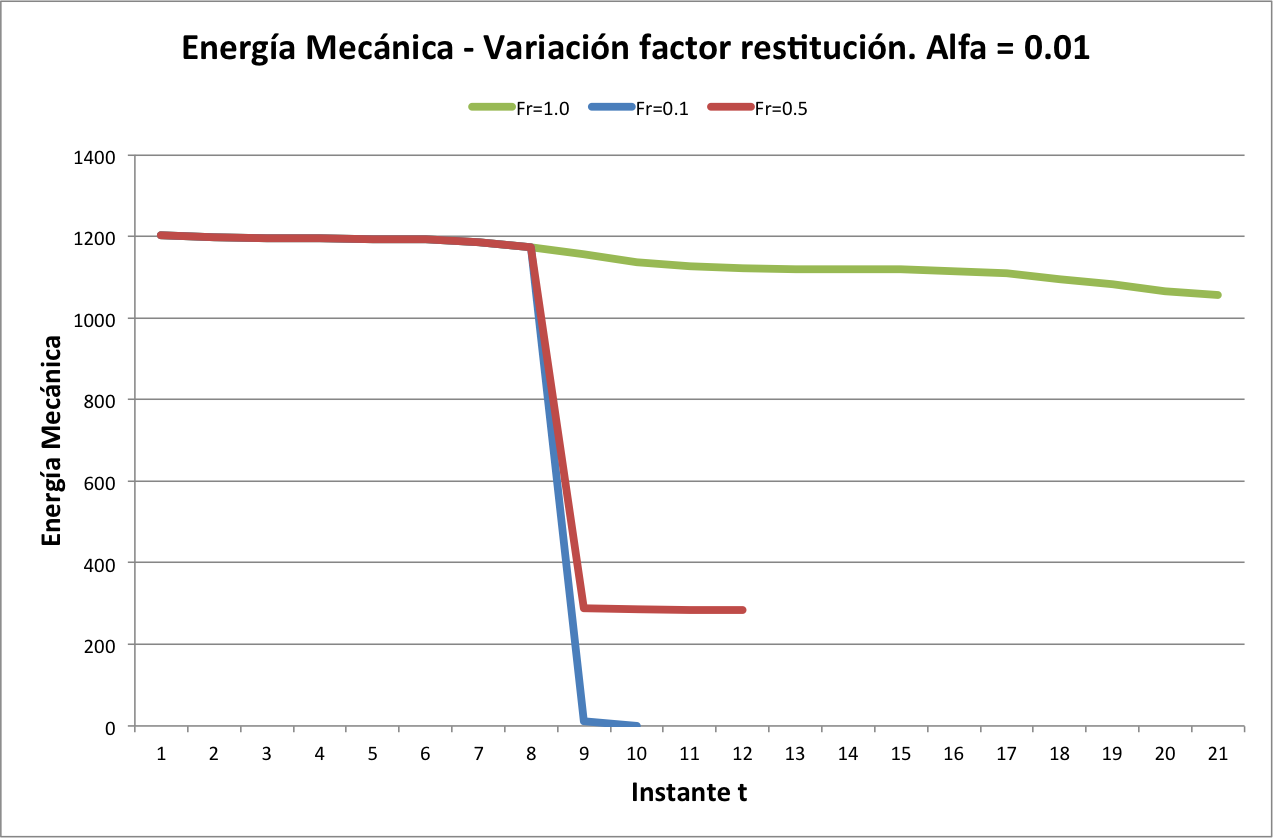
\includegraphics[scale=0.75]{graficos/5-energiaMecanica-fr.png}
  \caption{Comparación diferencia de energía mecánica. Variando \textit{Fr}. \texttt{Configuración A} }
\end{figure}
 	
En la \texttt{Figura 5} lo que hicimos fue, dejando fijo el $\alpha$, modificar el factor de restitución para ver como variaba la energía en este caso. Como era de esperar se puede observar que en el momento de los rebotes, a menor factor de restitución mayor pérdida de energía.\\[1em]


Como bien aclaramos antes, los resultados que mostramos hasta el momento utilizan una precisión de 52 bits de mantisa. Para los siguientes experimentos, vamos a variar la precisión para demostrar los errores que se cometen al reducir la misma.\\[1em]


En la \texttt{Figura 6} graficaremos el error que se produce al tener una menor precisión de representación para los números de punto flotante en aritmetica finita. 
Como la clase \textit{TFloat}, alcanza su máxima representación con 52 bits de mantisa, este fue el valor que utilizamos para tomar como valor válido. Luego, fuimos decrementando la mantisa y ejecutando el problema para la \texttt{configuración B} pero con menor precisión y comparamos el error absoluto del momento del primer impacto. \\[1em]

\begin{figure}[H]
  \centering
  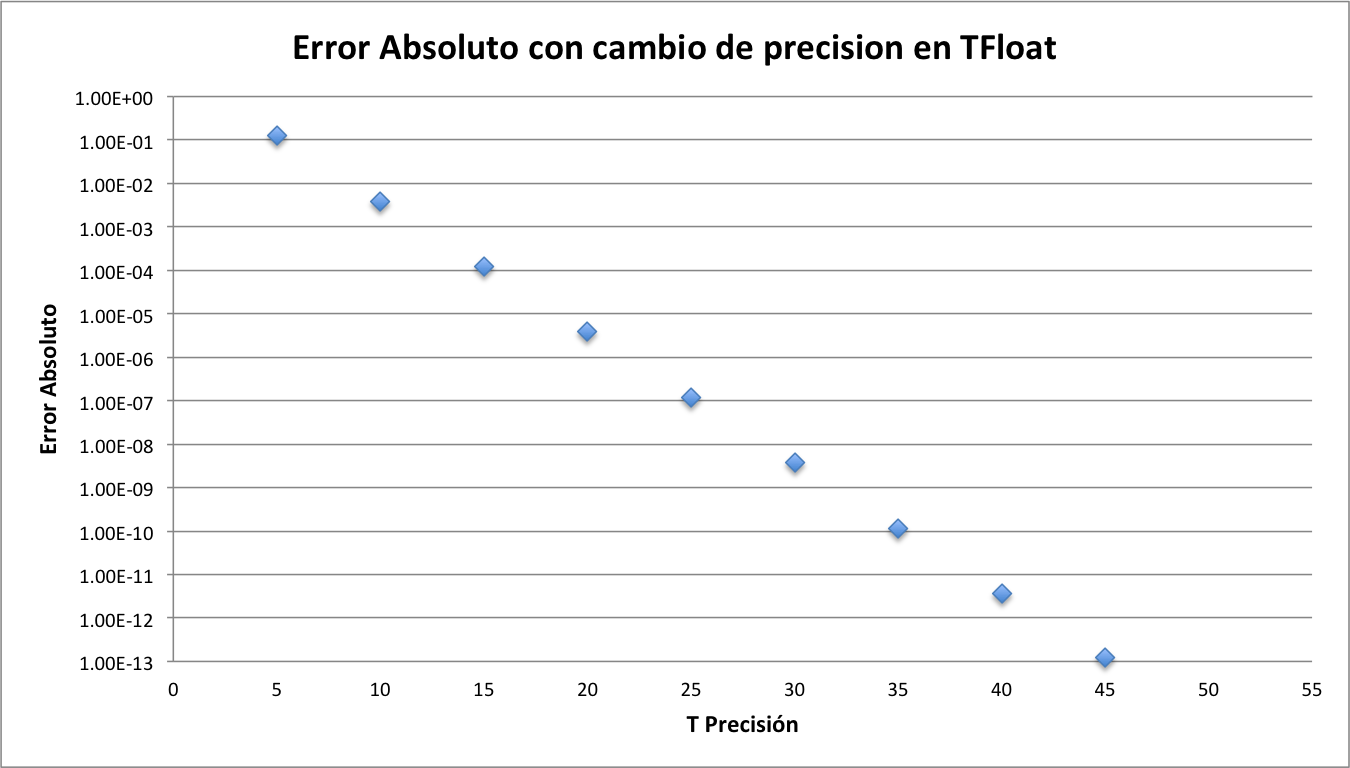
\includegraphics[scale=0.75]{graficos/6-errorAbsoluto.png}
  \caption{Error absoluto cambiando los bits de la mantisa. \texttt{Configuración B} }
\end{figure}

Luego de haber obtenido los resultados, los comparamos con nuestro \textit{valor ideal} y representamos la diferencia en la \texttt{Figura 6}.

Claramente una baja precisión aumenta el error en los cálculos.


En la siguiente \texttt{figura 7}, ejecutamos el mismo problema antes descrito modificando el \textit{factor de restitución} para mostrar como altera la altura máxima alcanzada luego del primer impacto.

\begin{figure}[H]
  \centering
  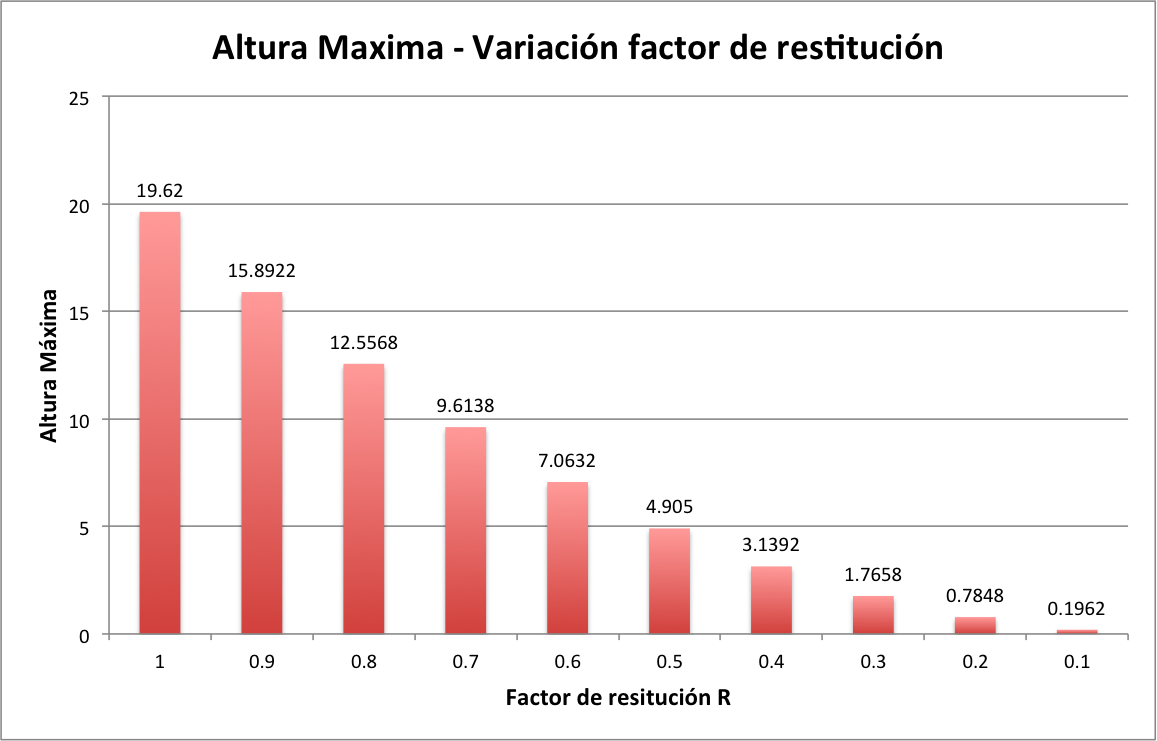
\includegraphics[scale=0.75]{graficos/7-AlturaMaxima-fr.png}
  \caption{Variando el factor de restitución, el impacto le quita velocidad y alcanza menores alturas. \texttt{Configuración B}}
\end{figure}

Como podemos observar, la altura máxima alcanzada cada vez es menor a medida que achicamos el factor de restitución, y esto debe porque luego del primer impacto, la velocidad con la que rebota se ve reducida por el mismo (siempre y cuando no consideremos la fricción para este experimento). Si en el experimento dejamos de lado el rozamiento, y el factor de restitución es 1 el objeto alcanzaría siempre la altura máxima y no dejaría de rebotar nunca.\\[1em]


Utilizando una vez mas el mismo caso de pruebas, decidimos analizar nuevamente la altura máxima pero esta vez modificando el coeficiente de rozamiento y mostrar como influye en lo que a este experimento se refiere. \texttt{Figura 8}.

\begin{figure}[H]
  \centering
  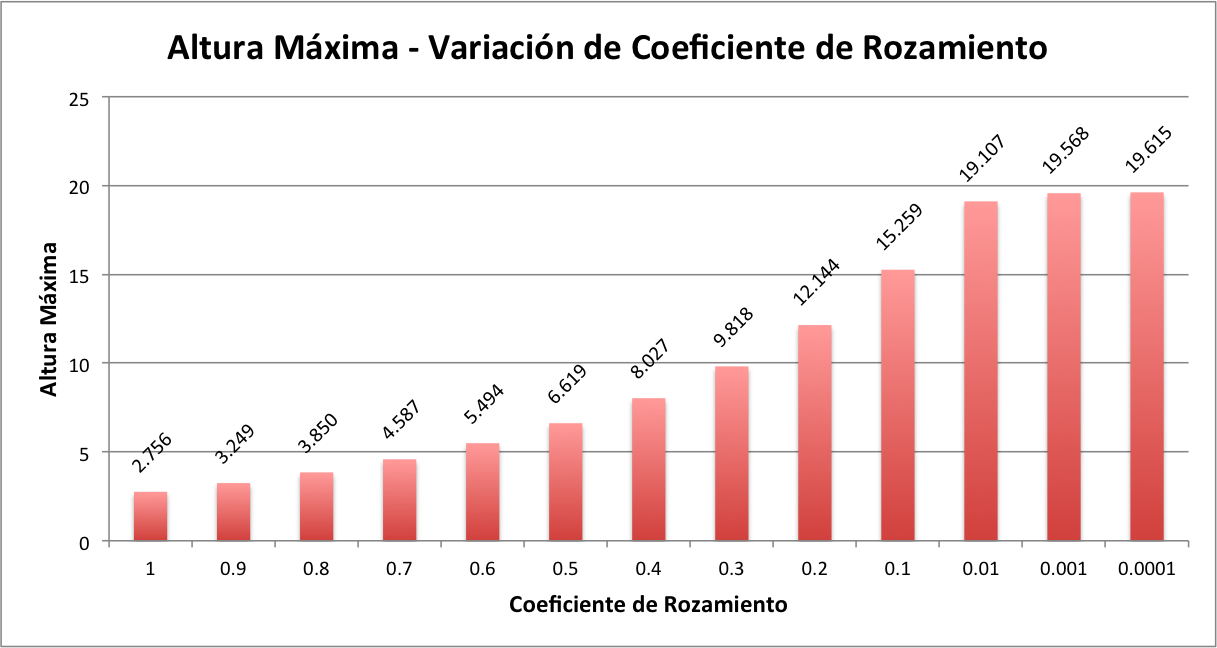
\includegraphics[scale=0.75]{graficos/8-AlturaMaxima-cr.png}
  \caption{Variamos el \textit{Cr} y evaluamos la altura máxima alcanzada. Manteniendo M=1. \texttt{Configuración B}}
\end{figure}

El \textbf{coeficiente de rozamiento o de fricción} expresa la oposición al deslizamiento que ofrece el objeto con, en este problema, el aire. En la \texttt{Figura 8} se puede apreciar como la altura máxima va aumentando debido a que tiene menor coeficiente de fricción, y por lo tanto la resistencia al deslizamiento cada vez es menor.



%Deben incluir los resultados de los experimentos, utilizando el formato m ́as adecuado para su presentaci ́on. Deber ́an especificar claramente a qu ́e experiencia corresponde cada resultado. No se incluir ́an aqu ́ı corridas de m ́aquina. Algo fundamental en su aprendizaje en la materia es la presentaci ́on de resultados de forma clara y concisa para el lector.
\newpage

%\section{Discusión}
%Se incluira aquı un analisis de los resultados obtenidos en la seccion anterior (se analizara su validez, coherencia, etc.). Deben analizarse como mınimo los ıtems pedidos en el enunciado. No es aceptable decir que “los resultados fueron los esperados”, sin hacer clara referencia a la teor ́ıa a la cual se ajustan. Adem ́as, se deben mencionar los resul- tados interesantes y los casos “patol ́ogicos” encontrados.

\subsection{Historial de Convergencia}

\begin{figure}[H]
  \centering
  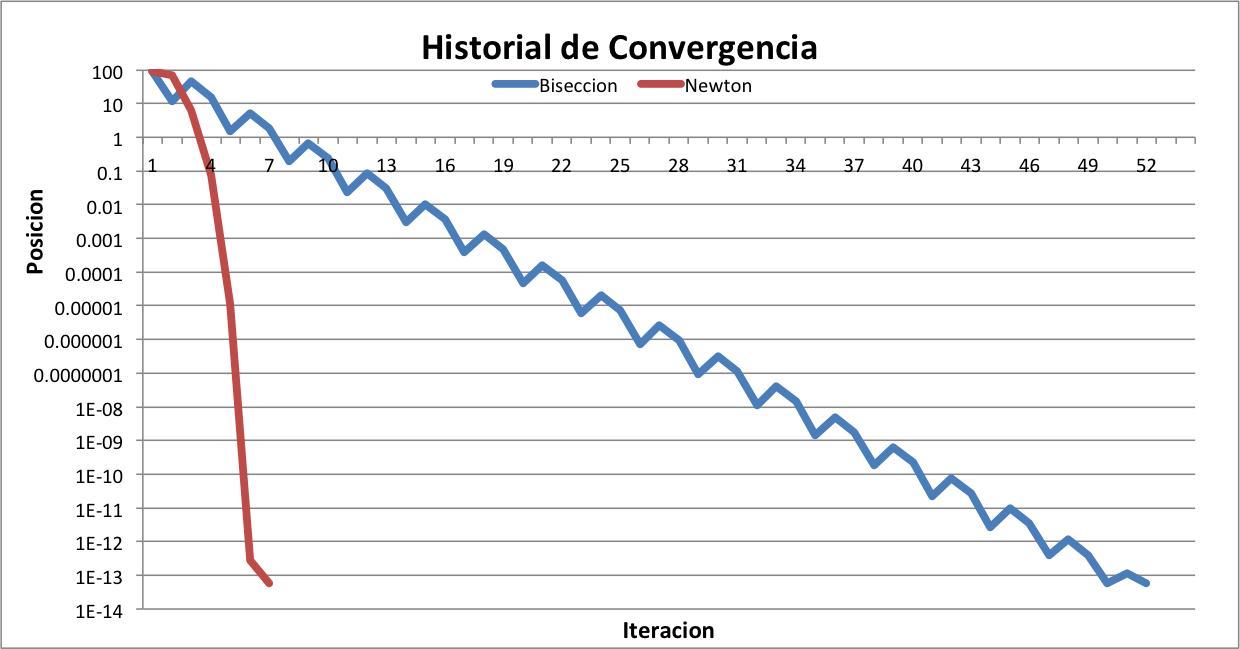
\includegraphics[scale=0.75]{graficos/9-HistorialConvergencia1.png}
  \caption{Diferencia absoluta de la posición de cada iteración con la posición de impacto (0) \texttt{Configuración A}}
\end{figure}

En la \texttt{Figura 9} se nota la velocidad con la que convergen los algoritmos, y plasma la diferencia teórica en cuanto la convergencia cuadrática de \textbf{Newton} y la convergencia lineal de \textbf{Bisección}.

Si bien \textbf{Bisección} muestra unos ciclos en el historial de convergencia, estos se mantienen dentro de la linealidad del algoritmo. La explicación que le encontramos a estos ciclos es debido a la particularidad del algoritmo, que depende de que lado de la raíz estemos evaluando la función y esto produce pequeños saltos cuando cambiamos de borde. 

\begin{figure}[H]
  \centering
  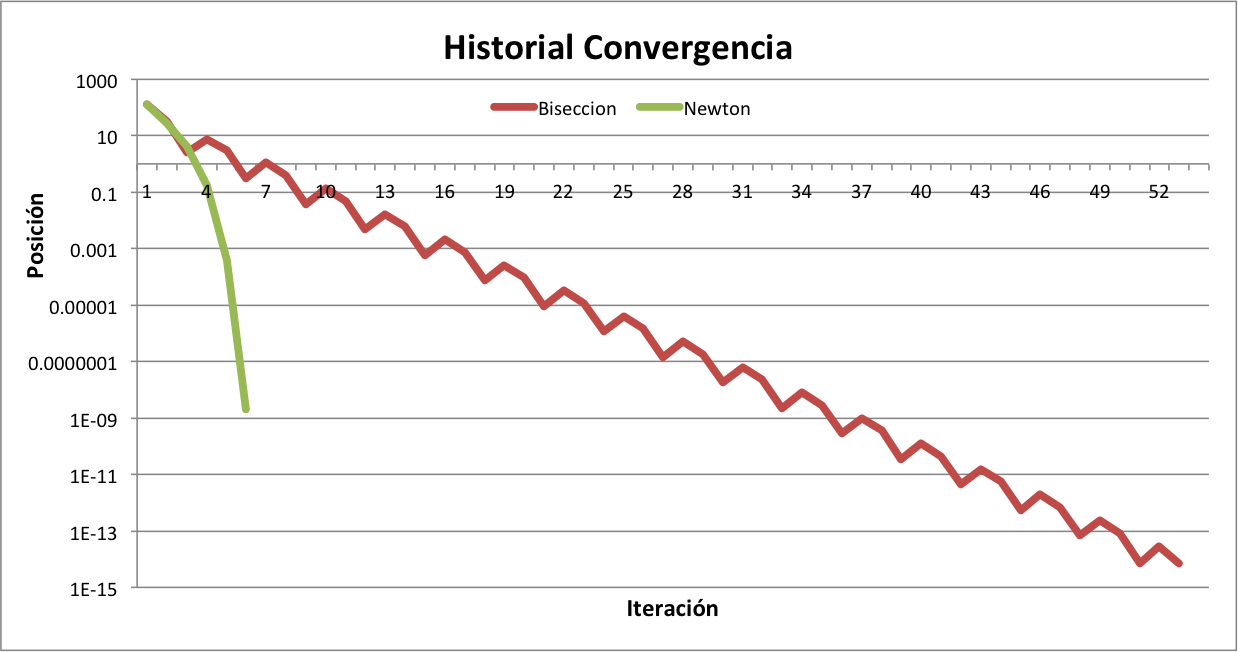
\includegraphics[scale=0.75]{graficos/10-HistorialConvergencia2.png}
  \caption{Diferencia absoluta de la posición de cada iteración con la posición de impacto (0) \texttt{Configuración B}}
\end{figure}

En esta última, \texttt{figura 10}, encontramos el mismo comportamiento explicado anteriormente, a diferencia que \textbf{Newton} da saltos más grandes y llega al cero antes, pero esto se debe a la configuración inicial. Como estos gráficos están en escala logarítmica el cero no puede ser representado entonces dejamos de graficar \textbf{Newton} una iteración antes de llegar al cero.

\newpage

\section{Conclusiones}
%Esta secci ́on debe contener las conclusiones generales del trabajo. Se deben mencionar las relaciones de la discusi ́on sobre las que se tiene certeza, junto con comentarios y observaciones generales aplicables a todo el proceso. Mencionar tambi ́en posibles extensiones a los m ́etodos, experimentos que hayan quedado pendientes, etc.
La implementación de métodos numéricos no es una tarea simple. En nuestro problema nos dimos cuenta que el resultado depende mucho de la aritmética finita de las computadoras. \\ \hspace{1em}
Por esto, nos vimos obligados a calcular a mano, varios resultados a los problemas para averiguar si la solución arrojada por los métodos era correcta y cuanto error estábamos cometiendo, incluyendo el error de representación.  \\ \vspace{1em}

En cuanto a los métodos, nos dimos cuenta de que lo mejor era aplicar una combinación de los mismos. Aplicando solo \textit{Bisección} si bien nos aseguramos la convergencia, el orden de la misma es lineal. Por otro lado \textit{Newton} no asegura la convergencia, pero en el caso de hacerlo, nos provee de un orden cuadrático. 
Primero ejecutamos \textit{Bisección} una cantidad de veces para obtener una 'buena' semilla para el método de \textit{Newton}. En nuestro caso no hacia falta obtener una semilla demasiado cerca del valor de la raíz, pero eso depende de cada problema en particular. 

Cierto es que nos concentramos en la resolución de los algoritmos, y de la aplicación de los métodos para el problema y no le dedicamos más tiempo al análisis de la variación de la precisión en números de punto flotante.

\newpage

\section{Apéndices}
\subsection{A - Enunciado}
{\bf Introducción}

La manzana que golpeó la cabeza de Isaac Newton (1643 -- 1727) además de dejarle un lindo chichón, lo hizo reflexionar sobre las leyes de la mecánica clásica. Estas leyes se siguen utilizando aun en nuestros días para analizar el movimiento de cuerpos y partículas en situaciones donde la realidad se parece bastante a las hipótesis asumidas por las mismas, por ejemplo el movimiento del los planetas en el espacio o el desplazamiento de cuerpos a velocidades bajas respecto de la de la luz ($\sim 300.000$ km/s). En nuestro caso nos interesa estudiar la caída de objetos en la atmósfera terrestre.

Modelaremos el problema de caída de dos maneras diferentes. 
\begin{description}
 \item[Caída libre:] En este caso despreciamos los efectos del rozamiento con el aire y consideramos que la única fuerza que actúa sobre el cuerpo es la gravedad $g$. Así, para un cuerpo lanzado verticalmente desde una altura $h$, con una velocidad inicial $v_0$, en un sistema de referencia donde la coordenada vertical $y$ crece hacia arriba desde el suelo y la gravedad apunta hacia abajo, la posición del cuerpo estará dada en cada instante de tiempo por
\begin{equation}
 y(t) = h + v_0 t - \frac{g}{2} t^2,
\end{equation}
y la velocidad del mismo será
\begin{equation}
 \dot{y}(t) = v_0 - g t.
\end{equation}
 \item[Caída con rozamiento: ] En este caso asumiremos que hay una fuerza de rozamiento que tiende a detener el movimiento del cuerpo y que es proporcional y opuesta a la velocidad en cada instante dada por: $F_r = - c_r \dot{y}$ y llamaremos a $c_r$ coeficiente de rozamiento. En este caso, la posición del cuerpo estará dada por
\begin{equation}
 y(t) = h + \frac{v_0}{\alpha} + \frac{g}{\alpha^2} - \frac{g}{\alpha} t -\left( \frac{v_0}{\alpha} + \frac{g}{\alpha^2} \right) e^{-\alpha t},
\end{equation}
donde hemos abreviado escribiendo $\alpha = c_r / m$ y $m$ es la masa del cuerpo. Así, la velocidad será 
\begin{equation}
 \dot{y}(t) = - \frac{g}{\alpha} +\left( v_0 + \frac{g}{\alpha} \right) e^{-\alpha t}.
\end{equation}
\end{description}

El impacto contra el suelo se produce cuando $y=0$. En caso que se desee estudiar el comportamiento luego del impacto se puede considerar que el cuerpo ``rebota'' en el suelo de manera no elástica tal que la velocidad inmediatamente después del rebote es 
\begin{equation}
\dot{y}(t_{impacto+}) = - f_r \, \dot{y}(t_{impacto-})
\end{equation}
donde $0 \leq f_r \leq 1$ se llama factor de restitución y toma en cuenta los efectos no elásticos del rebote. En este caso, $f_r = 1$ implica que el rebote fue completamente elástico.


{\bf Enunciado}

En este trabajo práctico se deberá hacer un programa que, dadas las características del cuerpo (masa y coeficiente de rozamiento) y las condiciones iniciales (altura y velocidad de lanzamiento) calcule el momento en que se produce el primer impacto contra el suelo y la velocidad en ese instante. Asumir que la aceleración de la gravedad es $g = 9.81$ m/s$^2$.

Utilizando este programa:
\begin{enumerate}
  \item Analizar el efecto de la precisión numérica utilizada y las tolerancias adoptadas en la solución obtenida al calcular el primer impacto.
  
  \item Considerar que luego del primer impacto el cuerpo ``rebota'' en el suelo de manera no elástica, calcular la altura máxima del objeto luego del primer rebote y el momento del segundo impacto.

  \item ¿Cómo varía la energía mecánica ($E = g y +\dot{y}^2/2$) del cuerpo entre el lanzamiento y el segundo rebote? Estudiar el efecto de $\alpha$ (donde $\alpha = 0$ implica considerar el caso sin rozamiento), $f_r$ y la precisión numérica en esta variación.
\end{enumerate}

\newpage

\subsection{B - Códigos Fuente}

\subsubsection{Stopping criteria}
\begin{verbatim}
bool stopping_criteria(double a, double b, double tolerance) {
  return fabs(a - b) < tolerance;
}
\end{verbatim}

\subsubsection{Bisección}
\begin{verbatim}
Result zero_bisection(Params *p, double (*fn)(Params *, double)) {
  int  iteracion = p->max_iterations;
  double a = p->a, b = p->b, m;
  Result res;

  while( --iteracion > 0 && !stopping_criteria(a,b, p->tolerance)) {
     res.zero = (b+a)/2;
    ( fn(p,a) * fn(p, res.zero) > 0 )? a = res.zero : b =  res.zero;
  }

  return res;
}
\end{verbatim}


\subsubsection{Newton-Raphson}
\begin{verbatim}
Result zero_newton(Params* p, double (*fn)(Params *, double), double (*deriv) (Params *, double)){
  double current = p->x, previous = 0.0;
  Result res;

  for(int i = p->max_iterations; i > 0 && !stopping_criteria(previous, current, p->tolerance); i--){
    previous = current;
    current = previous - (fn(p, previous)/deriv(p, previous));
  }

  res.speed = deriv(p,current);
  res.zero  = current;

  return res;
}
\end{verbatim}

\newpage

\subsection{C - Cómo compilar y usar el TP}
El directorio del TP contiene un Makefile, con lo cual para compilarlo basta sólamente con ejecutar \textbf{make}. Los binarios generados son: 

\begin{itemize}
  \item \textbf{tp} Calcula primer impacto, altura máxima y segundo impacto.
  \item \textbf{mechanical\_energy} Para ver la variación de la energía mecánica. Utiliza metodos de bisección.
\end{itemize}

Y reciben los siguientes parámetros:

\begin{description}
\item[-M] es el método a ejecutar y se mapean del siguiente modo:
\begin{itemize}
  \item 0 para Bisección
  \item 1 para Bisección con fricción
  \item 2 para Newton
  \item 3 para Newton con fricción
  \item 4 para Bisección + Newton
  \item 5 para Bisección + Newton con fricción
\end{itemize}
\item[-h] posición inicial.
\item[-v] velocidad inicial.
\item[-t] tolerancia para Bisección.
\item[-m] masa de la pelota.
\item[-c] coeficiente de rozamiento.
\item[-f] factor de restitución.
\item[-i] cantidad máxima de iteraciones.
\item[-a] borde inicial del intervalo.
\item[-b] borde final del intervalo.
\item[-x] valor inicial para Newton.
\item[-z] tolerancia para Newton.
\end{description}

\subsection{Corrección de Código}
\begin{itemize}
	\item El print estaba mal, utilizaba un \textbf{.dbl()} cuando no correspondía y el compilador no nos notificaba sobre eso.
	\item Problema al calcular el segundo rebote. Se llamaba la función posición en lugar de la de velocidad.
\end{itemize}


%\section{Referencias TODO}
%Es importante incluir referencias a libros, art ́ıculos y p ́aginas de Internet consultados durante el desarrollo del trabajo, haciendo referencia a estos materiales a lo largo del informe. Se deben citar tambi ́en las comunicaciones personales con otros grupos.



\end{document}
